% ---------------------------------------------------------------------------------------------------------------
% Name:         main.tex
% Author:      shibata seiya , Yusuke Kato , Atsushi Kuwagata , Takumi Shimada
% Created:     	Nov 26, 2019
% Last Date:   	Dec  15, 2019
% Note:        Advanced robot design and production's group report
% -------------------------------------------------------------------------------------------------------------

\documentclass[11pt,a4paper]{jsarticle}
\usepackage{amsmath,amssymb}
\usepackage{bm}
\usepackage[dvipdfmx]{graphicx}
\usepackage{graphicx}
\usepackage{ascmac}
%
\setlength{\textwidth}{\fullwidth}
\setlength{\textheight}{40\baselineskip}
\addtolength{\textheight}{\topskip}
\setlength{\voffset}{-0.2in}
\setlength{\topmargin}{0pt}
\setlength{\headheight}{0pt}
\setlength{\headsep}{0pt}

\makeatletter
\def\@maketitle{% 
\begin{center}% 
{\LARGE \@title \par}% タイトル 
\end{center}% 
\begin{flushright}% 
{\large \@date}% 日付 
\end{flushright}% 
\begin{flushright}% 
{\large \@author}% 著者 
\end{flushright}% 
\par\vskip 1.5em
}
%
%\newcommand{\divergence}{\mathrm{div}\,}  %ダイバージェンス
%\newcommand{\grad}{\mathrm{grad}\,}  %グラディエント
%\newcommand{\rot}{\mathrm{rot}\,}  %ローテーション
%
\title{2019年度ロボット設計製作特論\\発表後グループレポート\\
\LARGE  発表タイトル:ハンコを押すロボット}
%\leftline{加藤祐介 鍬形篤史 柴田生弥 島田拓海}
\author{1976007	加藤祐介 1976010	鍬形篤史\\1976016	柴田生弥 1976019	島田拓海}

\date{提出日\today}
\begin{document}
\maketitle
%
%
\section{概要}
本レポートは2019年度のロボット設計製作論におけるC班のグループレポートである.本講義課題は,音楽を扱うものまたは A + B = C を実施するロボットの製作を目的としたものである.C班はハンコを押すロボットを製作する(以下本プロジェクト).


本レポートでは,頑張りました。
\begin{itemize}
	\item 背景
	\item 目的
	\item メンバー構成と役割分担
	\item 開発方法
	\item ロボットの構成
	\item 活動記録
	\item 活動支援金の支出明細
\end{itemize}

についてまとめる.
\section{背景}
「ハンコ」の役割として"確かにこれに同意した"という意思表示の証拠として使われる認印がある.使用用途は様々で,郵便物や宅配物の受け取り,申請書,請求書,領収書などへの捺印がある.
許可証をたくさんハンコを押すのが面倒.
ロボットで簡単にロボットが押せる.
\section{目的}
簡単にハンコを押してくれるロボットの設計製作をおこなう.

\section{メンバーの構成と役割分担}
本プロジェクトのメンバーは3つの研究室のメンバーによって構成されており,各々の専門分野を持っている.
ロボットを開発するにあたり,表1のような構成で担当を決定した.
\begin{table}[htbp]
\begin{center}
\caption{Division of roles}  %ここにキャプションを入れると上につく。
\renewcommand{\tablename}{Table}
\begin{tabular}{|c|c|c|c|}
\hline
学生番号 &名前&担当箇所 \\ \hline\hline
1976007& 加藤祐介&リーダー,ソフトウェア実装\\ \hline
1976010& 鍬形篤史&メカ設計,ソフトウェア実装\\ \hline
1976016& 柴田生弥&ソフトウェア実装\\ \hline
1976019&島田拓海&メカ設計,メカ製作\\ \hline
\end{tabular}
%この下にキャプションをつけると,下につく。
\label{tbl:clock}
\end{center}
\end{table}

\section{方法}
週に一回ミーティングをおこない,タスク管理をしたよ.
\section{ロボットの構成}

\subsection{メカニズム}

%input image
\begin{figure}[htbp]
  \begin{center}
    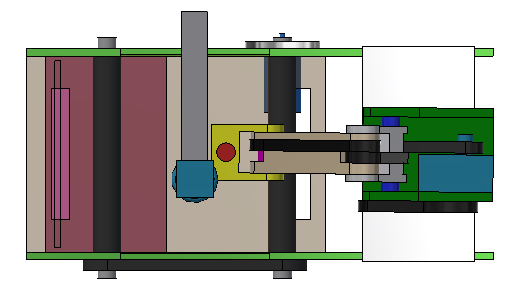
\includegraphics[width=10cm,height=6cm]{img/kitai.jpg}
    \caption{適当}
    \label{fig:one}
  \end{center}
\end{figure}

\subsection{回路とソフトウェア}

\section{結果}
こんな感じのできたよー

\section{活動記録}

\section{活動支出金}

\begin{table}[htbp]
\begin{center}
\caption{Division of roles}  %ここにキャプションを入れると上につく。
\renewcommand{\tablename}{Table}
\begin{tabular}{|c|c|c|c|c|c|c|}
\hline
購入日 &金額&商品名&型番&URL\\ \hline\hline
11/1& ¥8,335&サーマルプリンタ&&URL\\ \hline
11/18& 鍬形篤史&名前&名前&メカ設計,ソフトウェア実装\\ \hline
1976016& 柴田生弥&名前&名前&ソフトウェア実装\\ \hline
1976019&島田拓海&名前&名前&メカ設計,メカ製作\\ \hline
11/1& &名前&名前&URL\\ \hline
\end{tabular}
%この下にキャプションをつけると,下につく。
\label{tbl:clock}
\end{center}
\end{table}



%
%
\end{document}
